\documentclass[11pt, oneside]{article}   	% use "amsart" instead of "article" for AMSLaTeX format
\usepackage{geometry}                		% See geometry.pdf to learn the layout options. There are lots.
\geometry{letterpaper}                   		% ... or a4paper or a5paper or ... 
%\geometry{landscape}                		% Activate for rotated page geometry
\usepackage[parfill]{parskip}    		% Activate to begin paragraphs with an empty line rather than an indent
\usepackage{graphicx}				% Use pdf, png, jpg, or eps§ with pdflatex; use eps in DVI mode
								% TeX will automatically convert eps --> pdf in pdflatex		
\usepackage{caption}
\usepackage{subcaption}
\usepackage{float}
\usepackage{amssymb}
\usepackage{amsmath}
\usepackage{bm}
\usepackage{bbm}
\usepackage{mleftright}
\usepackage{todonotes}

\graphicspath{ {images/} }

\newcommand{\sotodo}{\todo[color=green]}
\newcommand{\sotodoinline}{\todo[color=green,inline=true]}
\newcommand{\bstodo}{\todo[color=pink]}
\newcommand{\bstodoinline}{\todo[color=pink,inline=true]}


%SetFonts

%SetFonts

\usepackage{natbib}
\usepackage{url}
%\bibliographystyle{elsarticle-harv}
\bibliographystyle{plain}

\newcommand{\half}{\frac{1}{2}}
\newcommand{\R}{\mathbb{R}}
\newcommand{\C}{\mathbb{C}}
\newcommand{\Z}{\mathbb{Z}}
\newcommand{\N}{\mathbb{N}}
\newcommand{\No}{\mathbb{N}_0}
\newcommand{\Ylm}{Y^m_l}
\newcommand{\Ylmfull}{Y^m_l(\theta,\varphi)}
\newcommand{\Plm}{P^m_l}
\newcommand{\costheta}{\cos\theta}
\newcommand{\sintheta}{\sin\theta}
\newcommand{\cosphi}{\cos\varphi}
\newcommand{\sinphi}{\sin\varphi}
\newcommand{\eimphi}{e^{im\varphi}}
\newcommand{\alphalm}{\alpha^m_l}
\newcommand{\clm}{c^m_l}
\newcommand{\ctilde}{\tilde{c}^m_l}
\newcommand{\ctildemod}{\tilde{c}^{|m|}_l}
\newcommand{\chat}{\hat{c}^m_l}
\newcommand{\chatmod}{\hat{c}^{|m|}_l}
\newcommand{\ddx}{\frac{\mathrm{d}}{\mathrm{d}x}}
\newcommand{\pddx}{\frac{\partial}{\partial x}}
\newcommand{\pddy}{\frac{\partial}{\partial y}}
\newcommand{\pddn}{\frac{\partial}{\partial n}}
\newcommand{\dmdxm}{\frac{\mathrm{d}^m}{\mathrm{d}x^m}}

\newcommand{\Atilde}{\tilde{A}_{l,m}}
\newcommand{\Btilde}{\tilde{B}_{l,m}}
\newcommand{\Dtilde}{\tilde{D}_{l,m}}
\newcommand{\Etilde}{\tilde{E}_{l,m}}
\newcommand{\Ftilde}{\tilde{F}_{l,m}}
\newcommand{\Gtilde}{\tilde{G}_{l,m}}
\newcommand{\Alm}{A_{l,m}}
\newcommand{\Blm}{B_{l,m}}
\newcommand{\Dlm}{D_{l,m}}
\newcommand{\Elm}{E_{l,m}}
\newcommand{\Flm}{F_{l,m}}
\newcommand{\Glm}{G_{l,m}}

\newcommand{\xione}{\xi^{(1)}_{n, \lambda}}
\newcommand{\xitwo}{\xi^{(2)}_{n, \lambda}}
\newcommand{\xithree}{\xi^{(3)}_{n, \lambda}}
\newcommand{\xifour}{\xi^{(4)}_{n, \lambda}}

\newcommand{\bigP}{\mathbb{P}}
\newcommand{\Pl}{\mathbb{P}_l}
\newcommand{\gradP}{T\mathbb{P}}
\newcommand{\gradPl}{T\mathbb{P}_l}
\newcommand{\gradY}{\nabla Y}
\newcommand{\gradYlm}{\nabla Y^m_l}
\newcommand{\gradpY}{\nabla^\perp Y}
\newcommand{\gradpYlm}{\nabla^\perp Y^m_l}

\newcommand{\Dlt}{D^\top_l}

\newcommand{\curlyy}{\bm{\mathcal{Y}}}
\newcommand{\blone}{\beta_{l, 1}}
\newcommand{\blzero}{\beta_{l, 0}}
\newcommand{\blmone}{\beta_{l, -1}}
\newcommand{\chivec}{\bm{\chi}_{1,m_s}}
\newcommand{\cgcoeff}{\mathcal{C}}

\newcommand{\alm}{a_{l,m}}
\newcommand{\blm}{b_{l,m}}
\newcommand{\dlm}{d_{l,m}}
\newcommand{\elm}{e_{l,m}}
\newcommand{\flm}{f_{l,m}}
\newcommand{\glm}{g_{l,m}}
\newcommand{\hlm}{h_{l,m}}
\newcommand{\jlm}{j_{l,m}}
\newcommand{\klm}{k_{l,m}}
\newcommand{\almperp}{a_{l,m}^\perp}
\newcommand{\blmperp}{b_{l,m}^\perp}
\newcommand{\dlmperp}{d_{l,m}^\perp}
\newcommand{\elmperp}{e_{l,m}^\perp}
\newcommand{\flmperp}{f_{l,m}^\perp}
\newcommand{\glmperp}{g_{l,m}^\perp}
\newcommand{\hlmperp}{h_{l,m}^\perp}
\newcommand{\jlmperp}{j_{l,m}^\perp}
\newcommand{\klmperp}{k_{l,m}^\perp}

\newcommand{\unitvec}{\hat{\bm{k}}}

\newcommand{\hdop}{H}
\newcommand{\bighdop}{\mathbb{\hdop}}
\newcommand{\hdopnk}{\hdop_{n,k}}
\newcommand{\hdopab}{\hdop^{(a,b)}}
\newcommand{\hdopnkab}{\hdop_{n,k}^{(a,b)}}
\newcommand{\Wab}{{W^{(a,b)}}}
\newcommand{\hdopmj}{\hdop_{m,j}}
\newcommand{\hdopmjab}{\hdop_{m,j}^{(a,b)}}
\newcommand{\alphaab}{\alpha^{(a,b)}}
\newcommand{\betaab}{\beta^{(a,b)}}
\newcommand{\bighdopab}{\bighdop^{(a,b)}}
\newcommand{\Dnt}{D^\top_n}
\newcommand{\Wii}{W^{(1,1)}}
\newcommand{\hdopii}{\hdop^{(1,1)}}
\newcommand{\bighdopii}{{\mathbb{\hdop}^{(1,1)}}}
\newcommand{\hdopoo}{\hdop^{(0,0)}}
\newcommand{\bighdopoo}{{\mathbb{\hdop}^{(0,0)}}}
\newcommand{\hdopoi}{\hdop^{(0,1)}}
\newcommand{\hdopio}{\hdop^{(1,0)}}
\newcommand{\genjac}{R}
\newcommand{\genjacnmk}{\genjac_{n-k}}
\newcommand{\genjacmmj}{\genjac_{m-j}}
\newcommand{\genjacw}{w_\genjac}
\newcommand{\normgenjac}{\omega_\genjac}
\newcommand{\normjac}{\omega_P}


\newcommand{\dx}{\frac{\partial}{\partial x}}
\newcommand{\dy}{\frac{\partial}{\partial y}}
\newcommand{\laplacewii}{\Delta_W^{(1,1)\to(1,1)}}
\newcommand{\laplacewtt}{\Delta_W^{(2,2)\to(0,0)}}
\newcommand{\laplaceoo}{\Delta^{(0,0)\to(2,2)}}
\newcommand{\biharmonic}{_2\Delta_W^{(2,2)\to(2,2)}}

\newcommand{\element}{\tau}
\newcommand{\refelement}{\hat{\tau}}
\newcommand{\FEset}{\mathcal{T}}
\newcommand{\bigW}{\mathbb{W}}
\newcommand{\bigWab}{\mathbb{W}^{(a,b)}}
\newcommand{\bigWii}{{\mathbb{W}^{(1,1)}}}
\newcommand{\bigQ}{\mathbb{Q}}
\newcommand{\bigQab}{\bigQ^{(a,b)}}

\usepackage{amsthm}

\newtheorem{proposition}{Proposition}
\newtheorem{lemma}{Lemma} 
\newtheorem{theorem}{Theorem} 
\newtheorem{definition}{Definition}
\newtheorem{algorithm}{Algorithm}

\include{somacros}

%\usepackage{media9}
%\graphicspath{ {../sphere/plots} }



\title{Sparse spectral and $p$-finite element methods for partial differential equations on disk-slices and trapeziums}
\author{Sheehan Olver, Ben Snowball}
%\date{}							% Activate to display a given date or no date


\begin{document}

\maketitle

\begin{abstract}
In recent years, sparse spectral methods for solving partial differential equations have been derived using hierarchies of classical orthogonal polynomials on intervals, disks, and triangles. In this work we extend this methodology to a hierarchy of non-classical orthogonal polynomials on disk slices (e.g. a half disk) and trapeziums. This builds on the observation that sparsity is guaranteed due to the boundary being defined by an algebraic curve, and that the entries of partial differential operators can be determined using formulae in terms of (non-classical) univariate orthogonal polynomials. 
\end{abstract}


%
\section{Introduction}

This paper develops sparse spectral methods for solving linear partial differential equations on a special class of geometries that includes disk slices and trapeziums.  
More precisely, we consider the solution of partial differential equations on the domain
\begin{align}
	\Omega := \{(x,y) \in \R^2 \quad | \quad \alpha < x < \beta, \: \gamma \rho(x) < y < \delta \rho(x)\}
\end{align}
where we require that either of the following scenarios hold:
\begin{enumerate}
\item  \(\rho\) is a degree 1 polynomial, or 
\item \(\rho\) is the square root of a non-negative degree \(\le\) 2 polynomial, \(-\gamma = \delta > 0\).
\end{enumerate}

For simplicity of discussion we focus in this paper on the half-disk, where $\rho(x) = \sqrt{1-x^2}$,  $(\alpha,\beta) = (0, 1)$, and  $(\gamma, \delta)  = (-1,1)$, with discussion of extension to other geometries in the appendix. 

We show that partial differential equations become sparse linear systems when viewed as acting on expansions involving a family of orthogonal polynomials (OPs) that  generalise Jacobi polynomials, mirroring the ultraspherical spectral method for ordinary differential equations \cite{olver2013fast} and its analogue on the triangle \cite{olver2018recurrence,olver2019triangle}.  On the half-disk the family of weights we consider are of the form
$$
W^{(a,b)}(x,y) = x^a (1-x-y)^b
$$
with corresponding OPs denoted $\hdopnkab(x,y)$, where $n$ denotes the polynomial degree, and $0 \le k \le n$. We define these to be orthogonalised lexicographically, that is,
$$
\hdopnkab(x,y) = C_{n,k} x^{n-k} y^k + (\hbox{lower order terms})
$$
where $C_{n,k} \neq 0$ and ``lower order terms'' can  include degree $n$ polynomials with fewer $y$ terms.

Sparsity comes from expanding the domain and range of an operator  using different choices of $a$ and $b$. Whereas the sparsity pattern and entries derived in \cite{olver2018recurrence,olver2019triangle} for equations on the triangle  results from manipulations of Jacobi polynomials, in the present work we use a more general integration-by-parts argument to deduce the sparsity structure, alongside quadrature rules to determine the entries.  Furthermore, we use this framework to derive sparse $p$-finite element methods that are analogous to those of Beuchler and Sch\"oberl on tetrahedra \cite{beuchler2006new}, see also work by Li and Shen \cite{li2010optimal}. 

The motivation for this work is solving partial differential equations on sub-domains of the sphere. In particular, OPs on a half-sphere can be represented using two families of OPs on the half-disk \cite[Theorem 3.1]{olver2018orthogonal}, where we would require $2n+1$ 3D OPs for each degree $n$, of which $n+1$ would be the $n+1$ degree $n$ OPs on the half-disk of the first family (polynomials in $x,y$) while the remaining $n$ OPs would be given by $z$ multiplied by the $n$ degree $n-1$ OPs on the half-disk of the second family. Constructing sparse spectral methods for surface PDEs on half-spheres, spherical caps, and spherical triangles is future work, and has applications in weather prediction. Other extensions include a full $hp$-finite element method on sections of a disk, which has applications in fluids. 

Here is an overview of the paper:  

\noindent \secref{OPs}: We present our procedure  to gain a (two-parameter) family of 2D orthogonal polynomials (OPs) on the half disk domain, by combining 1D OPs to the interval, to form 2D OPs on the disk. 

\noindent\secref{PDOs}: We demonstrate that these families will lead to sparse operators, including Jacobi operators representing multiplication by $x$ and $y$, and partial differential operators.

\noindent\secref{Computation}: We discuss computational issues, in particular, how to realise the results of the preceding sections in practice.  We  derive a quadrature rule on the half disk that can be used to expand a function in the OP basis up to a given order.  We implement function evaluation using the coefficients of the expansion of a given function using the Clenshaw algorithm.

\noindent\secref{Examples}: We demonstrate the proposed technique for solving Poisson, Helmholtz, and Biharmonic equations on the half-disk.  


\section{Orthogonal polynomials on the half disk}\label{Section:OPs}

In this section we outline the construction and some basic properties of $\hdopnkab(x,y)$. The symmetry in the weight allows us to express the polynomials in terms of 1D OPs, and deduce certain properties such as recurrence relationships. 

\subsection{Explicit construction}

By using a similar process to \cite[p55--56]{dunkl2014orthogonal} we can construct 2D orthogonal polynomials on $\Omega$ from 1D orthogonal polynomials on the intervals \([\alpha,\beta]\) and \([\gamma,\delta]\). We generalise this process to demonstrate a method of constructing multi-parameter families of 2D orthogonal polynomials on disk-slice and trapezium shaped domains $\Omega$ from multi-parameter families of 1D orthogonal polynomials on the intervals \([\alpha,\beta]\) and \([\gamma,\delta]\).

\begin{proposition}
Let \(w_1 : (\alpha,\beta) \: \to \R\), \(w_2 : (\gamma,\delta) \: \to \R\) be weight functions with \(\alpha,\beta,\gamma,\delta \in \R\), and let \(\rho \: : \: (\alpha,\beta) \: \to (0,\infty)\) be such that either:
\begin{enumerate}
\item  \(\rho\) is a degree 1 polynomial, or 
\item \(\rho\) is the square root of a non-negative degree \(\le\) 2 polynomial, \(-\gamma = \delta > 0\), and \(w_2\) is an even function.
\end{enumerate}
$\forall$, $n = 0,1,2,\dots, $ let $\{p_{n,k}\}$ be polynomials orthogonal with respect to the weight $\rho(x)^{2k+1} w_1(x)$ where $0 \le k \le n$, and $\{q_{n}\}$ be polynomials orthogonal with respect to the weight $w_2(x)$. Then the 2D polynomials defined on $\Omega$
$$
\hdopnk(x,y) := p_{n-k,k}(x) \: \rho(x)^k \: q_k\fpr(\frac{y}{\rho(x)}) \qquad\hbox{for} \qquad 0 \le k \le n, \: n = 0,1,2,\dots
$$
are orthogonal polynomials with respect to the weight \(W(x,y) := w_1(x) \: w_2(\frac{y}{\rho(x)}) \) on $\Omega$. 
\end{proposition}
\begin{proof}
See \cite[p55--56]{dunkl2014orthogonal}.
\end{proof}

We can generalise this for our purposes in the following proposition.
\begin{proposition}
Let
\begin{align*}
	\Omega := \{(x,y) \in \R^2 \quad | \quad \alpha < x < \beta, \: \gamma \rho(x) < y < \delta \rho(x)\}
\end{align*}
with $\rho : (\alpha, \beta) \to \R$. Further, let $\genjacw^{(a,b,c)}(x)$ and $w^{(a,b)}_P(x)$ be two weight functions on the intervals $(\alpha, \beta)$ and $(\gamma, \delta)$ respectively, given by:
\begin{align}
\begin{cases}
\genjacw^{(a,b,c)}(x) &:= (\beta - x)^a \: (x - \alpha)^{b} \: \rho(x)^{c} \\
w^{(a,b)}_P(x) &:= (\delta-x)^a \: (x - \gamma)^b
\end{cases}
\end{align}
where the three-parameter family of orthogonal polynomials on $[\alpha,\beta]$ given by $\{\genjac_n^{(a,b,c)}\}$ are orthogonal with respect to $\genjacw^{(a,b,c)}(x)$, and the two-parameter family of orthogonal polynomials on $[\gamma,\delta]$ given by $\{P_n^{(a,b)}\}$ are orthogonal with respect to $w^{(a,b)}_P(x)$.

Assume that either of the following hold:
\begin{enumerate}
\item  \(\rho\) is a degree 1 polynomial, or 
\item \(\rho\) is the square root of a non-negative degree \(\le\) 2 polynomial, \(-\gamma = \delta > 0\), and \(w^{(a,b)}_P\) is an even function (i.e. $a = b$, and we can hence denote the weight as $w^{(a)}_P(x) = (\delta-x^2)^a$).
\end{enumerate}
Then the four-parameter 2D polynomials defined on $\Omega$ given by
\begin{align}
	\hdopnk^{(a,b,c,d)}(x,y) := \genjacnmk^{(a, b, c+d+2k+1)}(x) \: \rho(x)^k \: P_k^{(d,c)}(\frac{y}{\rho(x)}), \quad (x,y) \in \Omega, 
\end{align}
are orthogonal polynomials with respect to the weight 
\begin{align}
	W^{(a,b,c,d)}(x,y) := \genjacw^{(a,b,c+d)}(x) \: w_P^{(d,c)}(\frac{y}{\rho(x)}), \quad (x,y) \in \Omega. 
\end{align}
\end{proposition}
\begin{proof}
See \cite[p55--56]{dunkl2014orthogonal}.
\end{proof}

For the half disk, the weight $W^{(a,b)}(x,y) = x^a \: (1-x^2-y^2)^b$ results from setting:
\begin{align}
\begin{cases}
(\alpha,\beta) &:= (0.1) \\
(\gamma,\delta) &:= (-1,1) \\
\rho(x) &:= (1-x^2)^{\half} \\
w_1(x) &:= \genjacw^{(a,b)}(x) := x^a \: (1-x^2)^b \\
w_2(x) &:= w_P^{(b)}(x) := (1-x^2)^b = (1-x)^b \: (1+x)^b,
\end{cases}
\end{align}
Note here the we have made the adjustment that $\genjacw^{(a,b,c)}(x) = (\beta - x)^a \: (x - \alpha)^{b} \: \rho(x)^{2c}$ and simply set the first parameter to zero and removed it for the specific half-disk case. This is for ease of writing and computation, by ensuring we reduce the need to incorporate unnecessary parameters and instead yield a two-parameter family of 2D orthogonal polynomials. 

The weight $w_2(x)$ is an ultraspherical weight, and the corresponding OPs are   the Jacobi polynomials  \(\{P_n^{(b, b)}\}\). The weight $w_1(x)$ is non-classical (it is in fact semi-classical, and is equivalent to a generalized Jacobi weight \cite[\S5]{magnus1995painleve}) and we introduce the notation \(\{\genjac_n^{(a, b)}\}\) for the orthonormal polynomials. Thus we arrive at  a two parameter family of 2D orthogonal polynomials $\{\hdopnkab\}$ given by, for $0 \le k \le n, \: n = 0,1,2,\dots,$
\begin{align}\label{eq:diskpolys}
 \hdopnk^{(a,b)}(x,y) := \genjacnmk^{(a, b+k+\half)}(x) \: \rho(x)^k \: P_k^{(b,b)}\fpr(\frac{y}{\rho(x)}), \quad (x,y) \in \Omega, 
\end{align}
orthogonal on \(\Omega\) with respect to the weight
\begin{align}
W^{(a,b)}(x,y) = \genjacw^{(a,b)}(x) \: w_P^{(b)}(\frac{y}{\rho(x)}) = x^a \: (1-x^2-y^2)^b.
\end{align}

The two 1D families of orthogonal polynomials we have denoted $\{\genjac_{n}^{(a,b)}\}$ and $\{P_n^{(b,b)}\}$ are not orthonormal, but have (squared) norms given by the integral of their respective weight functions we denote as
\begin{align}
	\normgenjac^{(a,b)} := \int_0^1 \: \genjacw^{(a,b)}(x) \: \D x, \quad \normjac^{(b)} := \int_{-1}^1 \: w_P^{(b)}(y) \: \D y,
\end{align}
i.e. $\norm{\genjac_{n}^{(a,b)}}_{\genjacw^{(a,b)}}^2 = \normgenjac^{(a,b)}$ $\forall n = 0,1,2,\dots$ and $\norm{P_{n}^{(b,b)}}_{w_P^{(b)}}^2 = \normjac^{(b)}$ $\forall n = 0,1,2,\dots$.

For clarity, we use the notation that 
\begin{align*}
&\ip<p, q>_{\genjacw^{(a,b)}} := \int_0^1 p(x) \: q(x) \: \genjacw^{(a,b)}(x) \: \D x, \quad
\ip<p, q>_{w_P^{(b)}} := \int_{-1}^1 p(y) \: q(y) \: w_P^{(b)}(y)\: \D y, \\
&\norm{p}_{\genjacw^{(a,b)}}^2 := \ip<p, p>_{\genjacw^{(a,b)}}, \quad
\norm{p}_{w_P^{(b)}}^2 := \ip<p, p>_{w_P^{(b)}}.
\end{align*}


\subsection{Jacobi matrices}

We can express the three-term recurrences associated to $\genjac_n^{(a,b)}$ and $P_n^{(b,b)}$ as
\begin{align}
x \genjac_n^{(a,b)}(x) &= \beta_n^{(a,b)} \genjac_{n+1}^{(a,b)}(x) + \alpha_n^{(a,b)} \genjac_n^{(a,b)}(x) + \beta_{n-1}^{(a,b)} \genjac_{n-1}^{(a,b)}(x) 
\label{eqn:Hrecurrence} \\
y P_n^{(b,b)}(y) &= \delta_n^{(b)} P_{n+1}^{(b,b)}(y) + \gamma_n^{(b)} P_n^{(b,b)}(y) + \delta_{n-1}^{(b)} P_{n-1}^{(b,b)}(y),
\end{align}
where we note that \(\gamma_n^{(b)} = 0\), for \( n = 0,1,2,\dots\). We can use these to determine the 2D recurrences for $\hdopnkab(x,y)$:

\begin{lemma}
$\hdopnk^{(a,b)}(x,y)$ satisfy the following 3-term recurrences:
\begin{align}
x \hdopnk^{(a,b)}(x,y) &= \alphaab_{n,k,1} \: \hdop_{n-1, k}^{(a,b)}(x, y) + \alphaab_{n,k,2} \: \hdop_{n, k}^{(a,b)}(x, y) + \alphaab_{n+1,k,1} \: \hdop_{n+1, k}^{(a,b)}(x, y), \\
y \hdopnk^{(a,b)}(x,y) &= \betaab_{n,k,1} \: \hdop_{n-1, k-1}^{(a,b)}(x, y) + \betaab_{n,k,2} \: \hdop_{n-1, k+1}^{(a,b)}(x, y) \nonumber \\
		& \quad \quad + \betaab_{n,k,3} \: \hdop_{n, k-1}^{(a,b)}(x, y) + \betaab_{n,k,4} \: \hdop_{n, k+1}^{(a,b)}(x, y) \nonumber \\
		& \quad \quad + \betaab_{n,k,5} \: \hdop_{n+1, k-1}^{(a,b)}(x, y) + \betaab_{n,k,6} \: \hdop_{n+1, k+1}^{(a,b)}(x, y),
\end{align}
for \((x,y) \in \Omega\), where
\begin{align}
\alphaab_{n,k,1} &:= \beta_{n-k-1}^{(a, b+k+\half)} \\
\alphaab_{n,k,2} &:= \alpha_{n-k}^{(a, b+k+\half)} \\
\betaab_{n,k,1} &:= \frac{\delta_{k-1}^{(b)}}{\normgenjac^{(a, b + k - \half)}} \: \ip<\genjacnmk^{(a, b+k+1/2)}, \genjacnmk^{(a, b+k-1/2)}>_{\genjacw^{(a, b+k+1/2)}} \\
\betaab_{n,k,2} &:= \frac{\delta_{k}^{(b)}}{\normgenjac^{(a, b + k + \frac{3}{2})}} \: \ip<\genjacnmk^{(a, b+k+1/2)}, \genjac_{n-k-2}^{(a, b+k+{3/2})}>_{\genjacw^{(a, b+k+{3/2})}} \\
\betaab_{n,k,3} &:= \frac{\delta_{k-1}^{(b)}}{\normgenjac^{(a, b + k - \half)}} \: \ip<\genjacnmk^{(a, b+k+1/2)}, \genjac_{n-k+1}^{(a, b+k-1/2)}>_{\genjacw^{(a, b+k+1/2)}} \\
\betaab_{n,k,4} &:= \frac{\delta_{k}^{(b)}}{\normgenjac^{(a, b + k + \frac{3}{2})}} \: \ip<\genjacnmk^{(a, b+k+1/2)}, \genjac_{n-k-1}^{(a, b+k+{3/2})}>_{\genjacw^{(a, b+k+{3/2})}} \\
\betaab_{n,k,5} &:= \frac{\delta_{k-1}^{(b)}}{\normgenjac^{(a, b + k - \half)}} \: \ip<\genjacnmk^{(a, b+k+1/2)}, \genjac_{n-k+2}^{(a, b+k-1/2)}>_{\genjacw^{(a, b+k+1/2)}} \\
\betaab_{n,k,6} &:= \frac{\delta_{k}^{(b)}}{\normgenjac^{(a, b + k + \frac{3}{2})}} \: \ip<\genjacnmk^{(a, b+k+1/2)}, \genjacnmk^{(a, b+k+{3/2})}>_{\genjacw^{(a, b+k+{3/2})}}. 
\end{align}

\end{lemma}

\begin{proof}
First, note that, using a change of variable,
\begin{align}
	\norm{\hdopnkab}_\Wab^2 &= \iint_\Omega \: {\genjacnmk^{(a,b+k+\half)}}(x)^2 \: \rho(x)^{2k} \: {P_k^{(b,b)}(\frac{y}{\rho(x)}}^2 \: \genjacw^{(a,b)}(x) \: w_P^{(b)}(\frac{y}{\rho(x)}) \: \D y \: \D x \nonumber \\
	&= \Big( \int_\alpha^\beta \: {\genjacnmk^{(a,b+k+\half)}}(x)^2 \: \genjacw^{(a,b+k+\half)}(x) \: \D x \Big) \: \Big( \int_\gamma^\delta \: {P^{(b,b)}}(y)^2 \: w_P^{(b)}(y) \: \D y \Big) \nonumber \\
	&= \normgenjac^{(a,b+k+\half)} \: \normjac^{(b)}.
\end{align}
where we use the notation that $\ip<p, q>_{\Wab} := \iint_\Omega p(x,y) \: q(x,y) \: \Wab(x,y) \: \D y \: \D x$ and $\norm{p}_{W^{(a,b)}}^2 := \ip<p, p>_{\Wab}$ .

Finally, note that \(\ip<y \hdopnkab, \hdopmjab>_\Wab = 0\) for \(m < n-1\) (and for \(m > n+2\)). Thus for \(m = n-1, n, n+1,\) \(j = 0,\dots,m:\)
\begin{align}
\ip<y \hdopnkab, \hdopmjab>_\Wab &=  \iint_\Omega \hdopnkab(x,y) \: \hdopmjab(x,y) \: y \: \Wab(x,y) \: dy \: dx \\
&= \Big( \int^1_0 \genjacnmk^{(a, b+k+\half)}(s) \: \genjacmmj^{(a, b+j+\half)}(s) \: s^a \: \rho(s)^{2b+k+j+2} \: ds \Big) \nonumber \\
& \quad \quad \quad\cdot \: \Big( \int^1_{-1} P_k^{(b,b)}(t) \: P_j^{(b,b)}(t) \: t \: (1-t^2)^b \: dt \Big) \\
&= \begin{cases}
    	\delta_k^{(b)} \: \normjac^{(b)} \: \ip<\genjacnmk^{(a, b+k+\half)}, \genjac_{m-k-1}^{(a, b+k+\frac{3}{2})}>_{\genjacw^{(a, b+k+\frac{3}{2})}} \quad& \text{if } j = k+1 \\
	\delta_{k-1}^{(b)} \: \normjac^{(b)} \: \ip<\genjacnmk^{(a, b+k+\half)}, \genjac_{m-k+1}^{(a, b+k-\half)}>_{\genjacw^{(a, b+k+\half)}} \quad& \text{if } j = k-1 \\
	0 & \text{otherwise}
      \end{cases}.
\end{align}

\end{proof}


Three-term recurrences lead to Jacobi operators that correspond to multiplication by $x$ and $y$. Define, for $n=0,1,2,\dots$: 
\begin{align}
\bighdopab_n := \begin{pmatrix}
		\hdopab_{n,0}(x,y) \\
		\vdots \\
		\hdopab_{n,n}(x,y)
	\end{pmatrix} \in \R^{n+1}, 
\quad \quad 
\bighdopab := \begin{pmatrix}
		\bighdopab_0 \\
		\bighdopab_1 \\
		\bighdopab_2 \\
		\vdots \\
	\end{pmatrix}
\end{align}
and set $J_x^{(a,b)}, J_y^{(a,b)}$ as the Jacobi matrices corresponding to
\begin{align}
J_x^{(a,b)} \: \bighdopab(x,y) = x \: \bighdopab(x,y), \quad J_y^{(a,b)} \: \bighdopab(x,y) = y \: \bighdopab(x,y).
\label{eqn:jacobimatricesdefinition}
\end{align}
The matrices $J_x^{(a,b)}, J_y^{(a,b)}$ act on the coefficients vector of a functions expansion in the $\{\hdopnkab\}$ basis. For example, let $a, b$ be general parameters and a function $f(x,y)$ defined on $\Omega$ be approximated by its expansion $f(x,y) = \bighdopab(x,y)^\top \mathbf{f}$. Then $x \: f(x,y)$ is approximated by $\bighdopab(x,y)^\top {J_x^{(a,b)\top}} \mathbf{f}$. In other words, ${J_x^{(a,b)\top}} \mathbf{f}$ is the coefficients vector for the expansion of the function $(x,y) \to x \: f(x,y)$ in the  $\{\hdopnkab\}$ basis.

$J_x^{(a,b)}, J_y^{(a,b)}$ have Banded-Block-Banded structures. A block-banded matrix is a block $n$-diagonal matrix where $n$ is reasonably small for the size of the full matrix. A banded-block-banded matrix is one where the blocks themselves are banded matrices. $J_x^{(a,b)}, J_y^{(a,b)}$ are given by:
\begin{align}
J_{x/y}^{(a,b)} &= \begin{pmatrix}
		B^{x/y}_0 & A^{x/y}_0 & & & & \\
		C^{x/y}_1 & B^{x/y}_1 & A^{x/y}_1 & & & \\
		& C^{x/y}_2 & B^{x/y}_2 & A^{x/y}_2  & & & \\
		& & C^{x/y}_3 & \ddots & \ddots & \\
		& & & \ddots & \ddots & \ddots \\
	\end{pmatrix}
\end{align}
where
\begin{align}
A^x_n &:= \begin{pmatrix}
		\alphaab_{n+1,0,1} & 0 & \hdots & 0 \\
		& \ddots & & \vdots & \\
		& & \alphaab_{n+1,n,1} & 0 \\
	    \end{pmatrix} \in \R^{(n+1)\times(n+2)}, \quad n = 0,1,2,\dots \\
B^x_n &:= \begin{pmatrix}
		\alphaab_{n,0,2} & & \\
		& \ddots & \\
		& & \alphaab_{n,n,2} \\
	    \end{pmatrix} \in \R^{(n+1)\times(n+1)} \quad n = 0,1,2,\dots \\
C^x_n &:= \big( A^x_n \big)^\top \in \R^{(n+1)\times n},  \quad n = 1,2,\dots \\ 
\nonumber \\
A^y_n &:= \begin{pmatrix}
		0 & \betaab_{n,0,6} & & & \\
		\betaab_{n,1,5} & 0 & & & \\
		& \ddots & \ddots & \ddots & \\
		& & \betaab_{n,n,5}& 0 & \betaab_{n,n,6} \\
	    \end{pmatrix} \in \R^{(n+1)\times(n+2)}, \quad n = 0,1,2,\dots \\
B^y_n &:= \begin{pmatrix}
		0 & \betaab_{n,0,4} & & \\
		\betaab_{n,1,3} & 0 & \ddots & \\
		& \ddots & \ddots & \betaab_{n,n-1,4} \\
		& & \betaab_{n,n,3} & 0
	    \end{pmatrix} \in \R^{(n+1)\times(n+1)}  \quad n = 0,1,2,\dots \\
C^y_n &:= \begin{pmatrix}
		0 & \betaab_{n,0,2} & & \\
		\betaab_{n,1,1} & 0 & \ddots & \\
		& \ddots & \ddots & \betaab_{n,n-2,2} \\
		& & \ddots & 0 \\
		& & & \betaab_{n,n,1} \\
	    \end{pmatrix} \in \R^{(n+1)\times n}, \quad n = 1,2,\dots
\end{align}

Note that the sparsity of the Jacobi matrices (in particular the sparsity of the sub-blocks) comes from the natural sparsity of the three-term recurrences of the 1D OPs, meaning that the sparsity is not limited to the specific half-disk case.




\subsection{Building the OPs} 

Combining each system in (\ref{eqn:jacobimatricesdefinition}) we can write the block-tridiagonal system
\begin{align}
\renewcommand\arraystretch{1.3}
\mleft[
\begin{array}{cccc}
		1 & & & \\
		B_0-G_0(x,y) & A_0 & & \\
		C_1 & B_1-G_1(x,y) & \quad A_1 \quad & \\
		& C_2 & \ddots & \ddots \\
		& & \ddots &
\end{array}
\mright]
\bighdopab(x,y)
=
\begin{pmatrix}
	P^{(a,b)}_{0,0} \\ 0 \\ 0 \\ \vdots \\ 0 \\
\end{pmatrix}.
\end{align}
where we note \(P^{(a,b)}_{0,0}(x,y) \equiv \genjac_0^{(a,b)} \: P_0^{(b,b)}\), and for each $n = 0,1,2\dots$:
\begin{align}
A_n &:= \begin{pmatrix}
		A^x_n \\
		A^y_n
	    \end{pmatrix} \in \R^{2(n+1)\times(n+2)} \quad (n \ne N), \quad
C_n := \begin{pmatrix}
		C^x_n \\
		C^y_n
	    \end{pmatrix} \in \R^{2(n+1)\times n} \quad (n \ne 0), \nonumber \\
B_n &:= \begin{pmatrix}
		B^x_n \\
		B^y_n
	    \end{pmatrix} \in \R^{2(n+1)\times(n+1)}, \quad
G_n(x,y) := \begin{pmatrix}
		xI_{n+1} \\
		yI_{n+1}
	    \end{pmatrix} \in \R^{2(n+1)\times(n+1)}.
\end{align}
 
For each $n = 0,1,2\dots$ let $\Dnt$ be any matrix that is a left inverse of $A_n$, i.e. such that $\Dnt A_n = I_{n+2}$. Multiplying our system by the preconditioner matrix that is given by the block diagonal matrix of the $\Dnt$'s, we obtain a lower triangular system \cite[p78]{dunkl2014orthogonal}, which can be expanded to obtain the recurrence:
\begin{align}
\begin{cases}
\bighdopab_{-1}(x,y) := 0 \\
\bighdopab_{0}(x,y) := P^{(a,b)}_{0,0} \\
\bighdopab_{n+1}(x,y) = -\Dnt (B_n-G_n(x,y)) \bighdopab_n(x,y) - \Dnt C_n  \,\bighdopab_{n-1}(x,y), \quad n = 1,2,3,\dots.
\end{cases}
\end{align}

Note that we can define an explicit \(\Dnt\) as follows. For \(n\) even:
\begin{align}
\Dnt := \begin{pmatrix}
		\frac{1}{\alphaab_{n+1,0,1}} & & &  \\
		& \ddots & & & \\
		& & \frac{1}{\alphaab_{n+1,n,1}} & \\
		0 & \hdots & 0 & \eta_{m-1} & \hdots & 0 & \eta_1 & 0 & \eta_0
	    \end{pmatrix},
\end{align}
where
\begin{align}
m &= \frac{n}{2} + 1, \quad \eta_0 = \frac{1}{\betaab_{n,n,6}},\qqand \nonumber \\
\eta_k &= -\frac{\betaab_{n,n-2(k-1),5} \: \eta_{k-1}}{\betaab_{n,n-2k,6}} \quad k = 1,\dots,m-1.
\end{align}

For \(n\) odd:

\begin{align}
\Dnt := \begin{pmatrix}
		\frac{1}{\alphaab_{n+1,0,1}} & &  \\
		& \ddots & & &  \\
		& & \ddots & & \\
		& & & \frac{1}{\alphaab_{n+1,n,1}} & \\
		\xi & 0 & \hdots & 0 & 0 & \eta_{m-2} & \hdots & 0 & \eta_0
	    \end{pmatrix},
\end{align}
 where
\begin{align}
m &= \frac{n+1}{2} + 1,\quad  \eta_0 = \frac{1}{\betaab_{n,n,6}}, \quad \xi = -\frac{\betaab_{n,1,5} \: \eta_{m-2}}{\alphaab_{n+1,0,1}},\qqand \nonumber \\
\eta_k &= -\frac{\betaab_{n,n-2(k-1),5} \: \eta_{k-1}}{\betaab_{n,n-2k,6}} \quad k = 1,\dots,m-2.
\end{align}
It follows that we can apply $\Dnt$ in $O(n)$ complexity, and thereby construct $\bighdopab_{n}(x,y)$ in optimal $O(n^2)$ complexity.

%
\section{Sparse partial differential operators}\label{Section:PDOs}


\begin{figure} 
\center
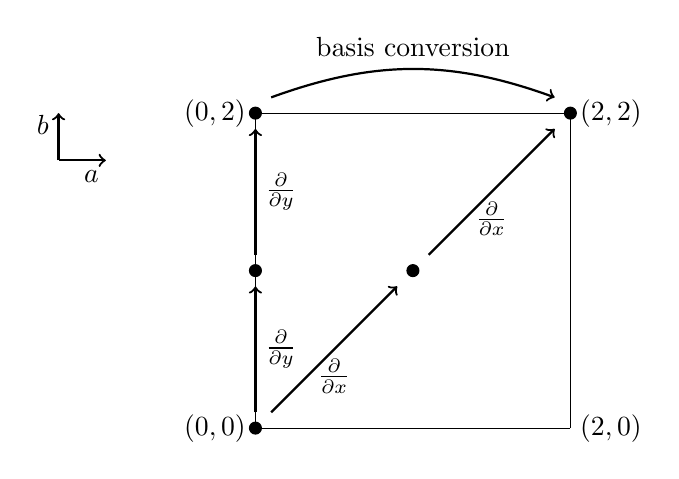
\begin{tikzpicture} 
% Box/square (4x4)
\draw[black,solid,ultra thin] (0,0)--(0,4);
\draw[black,solid,ultra thin] (0,0)--(4,0);
\draw[black,solid,ultra thin] (4,0)--(4,4);
\draw[black,solid,ultra thin] (0,4)--(4,4);
% Dots
\draw[black,fill=black] (0,0) circle (.5ex);
\draw[black,fill=black] (2,2) circle (.5ex);
\draw[black,fill=black] (4,4) circle (.5ex);
\draw[black,fill=black] (0,2) circle (.5ex);
\draw[black,fill=black] (0,4) circle (.5ex);
% Arrows
\draw[black,thick,->] (0.2,0.2)--(1.8,1.8);
\draw[black,thick,->] (2.2,2.2)--(3.8,3.8);
\draw[black,thick,->] (0,0.2)--(0,1.8);
\draw[black,thick,->] (0,2.2)--(0,3.8);
\draw [black,thick,->] (0.2,4.2) to [out=20,in=160] (3.8,4.2);
% Node (parameter) labels
\draw[] (0,0) node[anchor=east] {$(0,0)$};
\draw[] (0,4) node[anchor=east] {$(0,2)$};
\draw[] (4,0) node[anchor=west] {$(2,0)$};
\draw[] (4,4) node[anchor=west] {$(2,2)$};
% Arrow labels
\draw[] (1,1) node[anchor=north] {$\tfrac{\partial}{\partial x}$};
\draw[] (3,3) node[anchor=north] {$\tfrac{\partial}{\partial x}$};
\draw[] (0,1) node[anchor=west] {$\tfrac{\partial}{\partial y}$};
\draw[] (0,3) node[anchor=west] {$\tfrac{\partial}{\partial y}$};
% The key and headings
\draw[black,thick,->] (-2.5,3.4)--(-2.5,4);
\draw[black,thick,->] (-2.5,3.4)--(-1.9,3.4);
\draw[] (-2.3,3.2) node[anchor=west] {$a$};
\draw[] (-2.7,3.6) node[anchor=south] {$b$};
\draw[] (2,4.6) node[anchor=south] {basis conversion};
\end{tikzpicture} 
\caption{The Laplace operator acting on vectors of $\hdop_{n,k}=\hdop_{n,k}^{(0,0)}$ coefficients has a sparse matrix representation if the range is represented as vectors of $\smash{P^{(2,2)}_{n,k}}$ coefficients. Here, the arrows indicate that the corresponding operation has a sparse matrix representation when the domain is $\smash{\hdopnkab}$ coefficients, where $(a,b)$ is at the tail of the arrow, and the range is $\smash{\hdop_{n,k}^{(\tilde{a},\tilde{b})}}$ coefficients, where $(\tilde{a},\tilde{b})$ is at the head of the arrow. %For example, $\smash{\frac{\partial}{\partial x}}$ has a sparse matrix representation when the domain is represented in $\smash{\hdop_{n,k}^{(0,0,0)}}$ (resp.~$\smash{\hdop_{n,k}^{(1,0,1)}}$) and the range in $\smash{\hdop_{n,k}^{(1,0,1)}}$ (resp.~$\smash{\hdop_{n,k}^{(2,0,2)}}$).
}
\label{fig:Laplace} 
\end{figure}

Firstly, we introduce further notation that
\begin{align}
\bigWab(x,y) := \Wab(x,y) \bighdopab(x,y).
\end{align}

Recall that, for $a, b$ be general parameters, a function $f(x,y)$ defined on $\Omega$ is approximated by its expansion $f(x,y) = \bighdopab(x,y)^\top \mathbf{f}$. Recall also that $\Wab(x,y) := \genjacw^{(a,b)}(x) \: w_P^{(b)}(\frac{y}{\rho(x)})$, where $\rho(x) := (1-x^2)^\half$, $\genjacw^{(a,b)}(x) := x^a \: (1-x^2)^b$ and $w_P^{(b)}(y) := (1-y^2)^b$ for the half disk case.

There exist sparse operators \(D_x^{(a,b)}, \: D_y^{(a,b)}, \: W_x^{(a,b)}, \: W_y^{(a,b)}\) such that:
\begin{align}
{\partial f \over \partial x}&= \bighdop^{(a+1,b+1)}(x,y)^\top \: D_x^{(a,b)} \: \mathbf{f}, \\
{\partial f \over \partial y} &= \bighdop^{(a,b+1)}(x,y)^\top \: D_y^{(a,b)} \: \mathbf{f}, \\
{\partial \over \partial x}[\Wab(x,y) \: f(x,y)] &= \bigW^{(a-1,b-1)}(x,y)^\top \: W_x^{(a,b)} \: \mathbf{f}, \\
{\partial \over \partial y}[\Wab(x,y) \: f(x,y)] &= \bigW^{(a,b-1)}(x,y)^\top \: W_y^{(a,b)} \: \mathbf{f}.
\end{align}
The incrementing and decrementing of parameters as seen here is analogous to other well known orthogonal polynomials families' derivatives, for example the Jacobi polynomials on the interval, as seen in the DLMF \cite{DLMFDerivatives}, and on the triangle \cite{olver2018recurrence}.

Further, we note that there exist ``parameter transformation" Banded-Block-Banded matrix operators that increment/decrement the parameters, transforming the OPs from one (weighted or non-weighted) parameter space to another. We denote these operators as $T^{(a,b)\to(a+1,b)}$, $T^{(a,b)\to(a,b+1)}$ and $T^{(a,b)\to(a+1,b+1)}$ for conversion between non-weighted spaces, and similarly $T_W^{(a,b)\to(a-1,b)}$, $T_W^{(a,b)\to(a,b-1)}$ and $T_W^{(a,b)\to(a-1,b-1)}$ for conversion between weighted spaces, where:
\begin{align}
\bighdop^{(a,b)}(x,y) &= \Big(T^{(a,b)\to(a+1,b)} \Big)^\top \: \bighdop^{(a+1,b)}(x,y) \\
\bighdop^{(a,b)}(x,y) &= \Big(T^{(a,b)\to(a,b+1)} \Big)^\top \: \bighdop^{(a,b+1)}(x,y) \\
\bighdop^{(a,b)}(x,y) &= \Big(T^{(a,b)\to(a+1,b+1)} \Big)^\top \: \bighdop^{(a+1,b+1)}(x,y) \\
\bigW^{(a,b)}(x,y) &= \Big(T_W^{(a,b)\to(a+1,b)} \Big)^\top \: \bigW^{(a-1,b)}(x,y) \\
\bigW^{(a,b)}(x,y) &= \Big(T_W^{(a,b)\to(a,b+1)} \Big)^\top \: \bigW^{(a,b-1)}(x,y) \\
\bigW^{(a,b)}(x,y) &= \Big(T_W^{(a,b)\to(a+1,b+1)} \Big)^\top \: \bigW^{(a-1,b-1)}(x,y) \\
\end{align}

\begin{figure}
	\centering
	\begin{subfigure}[t]{0.3\textwidth}
	\centering
	\includegraphics[scale=0.35]{sparsityoflaplacian-w11}
	\end{subfigure}
	\begin{subfigure}[t]{0.3\textwidth}
	\centering
	\includegraphics[scale=0.35]{sparsityofhelmholtz}
	\end{subfigure}
	\begin{subfigure}[t]{0.3\textwidth}
	\centering
	\includegraphics[scale=0.35]{sparsityofbiharmonic}
	\end{subfigure}
    	\caption{"Spy" plots of (differential) operator matrices, showing their sparsity. Left: the Laplace operator $\laplacewii$. Centre: the weighted variable coefficient Helmholtz operator $\laplacewii + k^2 \: T^{(0,0)\to(1,1)} \: V({J_x^{(0,0)}}^\top, {J_y^{(0,0)}}^\top) \: T_W^{(1,1)\to(0,0)}$ for $v(x,y) = 1 - (3(x-1)^2 + 5y^2)$ and $k = 200$. Right: the biharmonic operator $\biharmonic$.}
        \label{fig:sparsity}
\end{figure}

We can then obtain the matrix operator for the Laplacian \(\Delta\), that will take us from coefficients for expansion in the weighted space
$$
\bigWii(x,y) = \Wii(x,y) \: \bighdopii(x,y)
$$
to coefficients in the non-weighted space $\bighdopii(x,y)$. Note that this construction will ensure the imposition of the Dirichlet zero boundary conditions on $\Omega$. The matrix operator for the Laplacian we denote $\laplacewii$ acting on the coefficients vector is then given by
\begin{align}
    \laplacewii := D_x^{(0,0)} \: W_x^{(1,1)} + T^{(0,1)\to(1,1)} \: D_y^{(0,0)} \: T_W^{(1,0)\to(0,0)} \: W_y^{(1,1)}.
\end{align}
Importantly, this operator will have Banded-Block-Banded structure, and hence will be sparse, as seen in Figure \ref{fig:sparsity}.

We can use the same technique for constructing a sparse Laplacian operator to construct the Biharmonic operator $\Delta^2$, that ensures we use a basis that satisfies both zero Dirichlet and Neumann conditions. On this note, we can also obtain the matrix operator for the Laplacian $\Delta$ that will take us from coefficients for expansion in the space $\bighdopoo(x,y)$ to coefficients in the space $\bighdop^{(2,2)}(x,y)$. We denote this matrix operator that acts on the coefficients vector as $\laplaceoo$, and is given by
\begin{align}
    \laplaceoo := D_x^{(1,1)} \: D_x^{(0,0)} + T^{(1,2)\to(2,2)} \: D_y^{(1,1)} \: T^{(0,1)\to(1,1)} \: D_y^{(0,0)}.
\end{align}
Further represent the Laplacian as a map from coefficients in the space $\bigW^{(2,2)}$ to coefficients in the space $\bighdopoo$. Note that a function expanded in the $\bigW^{(2,2)}$ basis will satisfy both zero Dirichlet and Neumann boundary conditions on $\Omega$. We denote this matrix operator as $\laplacewtt$, and is given by
\begin{align}
	\laplacewtt := W_x^{(1,1)} \: W_x^{(2,2)} + T_W^{(1,0)\to(0,0)} \: W_y^{(1,1)} \: T_W^{(2,1)\to(1,1)} \: W_y^{(2,2)}.
\end{align}
We can then construct a matrix operator for $\Delta^2$ that will take coefficients in the space $\bigW^{(2,2)}$ to coefficients in the space $\bighdop^{(2,2)}$. Note that any function expanded in the $\bigW^{(2,2)}$ basis will satisfy both zero Dirichlet and zero Neumann boundary conditions on $\Omega$. The matrix operator for the Biharmonic operator is then given by
\begin{align}
	\biharmonic = \laplaceoo \: \laplacewtt.
\end{align}
The sparsity and structure of this biharmonic operator is seen in Figure \ref{fig:sparsity}.

The sparsity of the these operators can be shown using a simple integration by parts argument, see Section \ref{subsection:Computation-operatormatrices}.



\section{Computational aspects}\label{Section:Computation}

\subsection{Constructing $\genjac_n^{(a,b)}(x)$}

To obtain the recurrence coefficients for the $\{\genjac_n^{(a,b)}\}$ OPs in (\ref{eqn:Hrecurrence}), we use a version of the Stieltjes algorithm. Recall that
\begin{align}
x \genjac_n^{(a,b)}(x) &= \beta_n^{(a,b)} \genjac_{n+1}^{(a,b)}(x) + \alpha_n^{(a,b)} \genjac_n^{(a,b)}(x) + \beta_{n-1}^{(a,b)} \genjac_{n-1}^{(a,b)}(x), \quad n = 0,1,2,\dots
\end{align}
where we define $\beta_{-1}^{(a,b)} = 0$ and $H_{-1}^{(a,b)}(x) \equiv 0$. We use a variant of the Stieltjes procedure \cite{gautschi1982generating} where the polynomials are expressed as Chebyshev polynomial expansions and the inner products are calculated via Clenshaw--Curtis quadrature. This has the benefit that it is easier to incorporate high-precision arithmetic, which we use to overcome ill-conditioning present when $b$ is large, as required for large $n$ in \eqref{eq:diskpolys}. The ApproxFun.jl \cite{ApproxFun} package gives a convenient way to manipulate Chebyshev and Jacobi expansions, which we use to calculate the inner products and norms in this algorithm.


\subsection{Quadrature rules}

In this section we construct a quadrature rule exact for polynomials in $\Omega$ that can be used to expand functions in $\hdopnkab(x,y)$. 

\begin{theorem}

Denote the  Gauss quadrature nodes and weight on \([0,1]\) with weight \(s^a \: (1-s^2)^{b+\half}\) as $(s_k,w_k^{(s)})$ , and
 on \([-1,1]\) with weight \((1-t^2)^b\) as $(t_k,w_k^{(t)})$. Define
\begin{align}
x_{i+(k-1)N} &:= s_k, \quad i,k = 1,\dots,N, \\
y_{l+(i-1)N} &:= (1-s_l^2)^\half \: t_l, \quad i,l = 1,\dots,N, \\
w_{l+(k-1)N} &:= w_k^{(s)} w_l^{(t)}, \quad k,l = 1,\dots,N.
\end{align}
Let $f(x,y)$ be a polynomial on $\Omega$. The quadrature rule is then
$$
\iint_\Omega f(x,y) \: \Wab(x,y) \: \D A \approx \half \sum_{j=1}^{N^2} w_j \: \big[ f(x_j, y_j) + f(x_j, -y_j) \big],
$$
where if $f(\cdot, y)$ for fixed $y$ is an at most degree $N$ polynomial and $f(x, \cdot)$ for fixed $x$  is an at most degree $2N-1$ polynomial, the quadrature rule is exact.
\end{theorem}

\begin{proof}
We will use the substitution that
\begin{align}
x &= s, \quad y = (1-s^2)^\half t.
\end{align}
First, note that
\begin{align}
W^{(a,b)}(x,y) &= x^a \: (1-x^2-y^2)^b, \quad \text{for } (x,y) \in \Omega, \\
		      &= s^a \: (1-s^2)^{b} \: (1-t^2)^b =: V^{(a,b)}(s,t), \quad \text{for } (s,t) \in [0,1] \times [-1,1].
\end{align}
\end{proof}

Note here that due to the symmetry in the domain, the integral of an odd function in the second variable (i.e. if $f(x, \dot)$ is odd for fixed $x$) over $\Omega$ is zero. Thus, the quadrature rule is such that we only consider the even part of a function.



\subsection{Obtaining the coefficients for expansion of a function}

Fix \(a,b \in \R\). Then for any function \(f : \Omega \to \R\) of degree $N$ we can express \(f\) by
\begin{align*}
f(x,y) = \sum_{n=0}^N \bighdop_n^{(a,b)}(x,y)^\top \: \mathbf{f}_n
\end{align*}
where
\begin{align*}
\bighdop_n(x,y) &:= \begin{pmatrix}
		\hdop_{n,0}(x,y) \\
		\vdots \\
		\hdop_{n,n}(x,y)
	\end{pmatrix} \in \R^{n+1} \quad \forall n = 0,1,2,\dots,N,
\end{align*}
and where
\begin{align*}
\mathbf{f}_n &:= \begin{pmatrix}
		f_{n,0} \\
		\vdots \\
		f_{n,n}
	\end{pmatrix} \in \R^{n+1} \quad \forall n = 0,1,2,\dots,N, \quad
f_{n,k} := \frac{\langle f, \: \hdopnk^{(a,b)} \rangle_{W^{(a,b)}}}{|| \hdopnk^{(a,b)} ||_{W^{(a,b)}}}
\end{align*}

Using the quadrature rule detailed in Section 4.2, we can calculate exactly the coefficients $f_{n,k}$: 
\begin{align}
	\ip< f, \: \hdopnk^{(a,b)} >_{W^{(a,b)}} &= \half \: \sum_{j=1}^{N^2} w_j \: \big[ f(x_j, y_j) \: \hdopnk^{(a,b)}(x_j, y_j) +f(x_j, -y_j) \: \hdopnk^{(a,b)}(x_j, -y_j) \big], \\
	|| \hdopnk^{(a,b)} ||_{W^{(a,b)}}^2 &= \half \: \sum_{j=1}^{N^2} w_j \: \big[ \hdopnk^{(a,b)}(x_j, y_j)^2 + \hdopnk^{(a,b)}(x_j, -y_j)^2 \big].
\end{align}

%\bstodo{This section contains repetition / expansion on the quadrature rule section above - not sure if we should remove it or move it?} We can develop a quadrature rule on the half disk \(\Omega\) in order to evaluate (40) and obtain the coefficient vectors \(\mathbf{f}_n\) as follows.
%
%Let \(f(x,y)\) be polynomial that is even in \(y\) of degree $d_1$ in $x$ and degree $d_2$ in $y$ (i.e. $f(\cdot, y)$ with $y$ fixed is a degree $d_1$ polynomial, and $f(x, \cdot)$ with $x$ fixed is an even degree $d_2$ polynomial). Then there exists a polynomial \(\tilde{f}(x,y)\) in \(x,y\) such that \(g(s,t) := f(x, y) = f(s, (1-s^2)^\half t) = \tilde{f}(s, (1-s^2) t^2)\) (i.e. that $d_2$ is an even integer). Now, as \(\tilde{f}\) is a polynomial, so must \(g\) be a polynomial of degree $d_1+\frac{d_2}{2}$ in $s$ and degree $d_2$ in $t$. Thus a quadrature rule of the following will be exact for the polynomial $f(x,y)$ (even in \(y\) of degree $\le d_1$ in $x$ and degree $\le d_2$ in $y$):
%\begin{align}
%& \quad \int_0^1 \int_{-\rho(x)}^{\rho(x)} W^{(a,b)}(x,y) \: f(x,y) \: dy \: dx \\
%&= \int_0^1 \int_{-1}^1 V^{(a,b)}(s,t) \: g(s,t) \: (1-s^2)^\half \: dt \: ds \\
%&= \int_0^1 s^a \: (1-s^2)^{b+\half} \: \Big( \sum_k^{\half(d_2 + 1)} w_k^{(t)} \: g(s, t_k) \Big) \: ds \\
%&= \sum_j^{\half(d_1 + \frac{d_2}{2} + 1)} \sum_k^{\half(d_2 + 1)} w_j^{(s)} w_k^{(t)} \: g(s_j, t_k) \\
%&= \sum_j^{\half(d_1 + \frac{d_2}{2} + 1)} \sum_k^{\half(d_2 + 1)} w_j^{(s)} w_k^{(t)} \: f(x_j, y_{j,k}),
%\end{align}
%where \(x_j := s_j,\) \(y_{j,k} := \rho(s_j) \: t_k\) are the quadrature points.
%
%We further note that for any polynomial \(f(x,y)\) that is odd in \(y\),
%\begin{align}
%\int_0^1 \int_{-\rho(x)}^{\rho(x)} W^{(a,b)}(x,y) \: f(x,y) \: dy \: dx = 0.
%\end{align}
%
%
%Then our quadrature rule for any polynomial \(f(x,y)\) on \(\Omega\) is:
%\begin{align}
%\int \int_\Omega W^{(a,b)}(x,y) \: f(x,y) \: dy \: dx \approx \half \: \sum_{j=1}^{N^2} w_j \: \big[ f(x_j, y_j) + f(x_j, -y_j) \big],
%\end{align}
%and is exact for any polynomial $f(x,y)$ where the degree in $x$ is $\le N$ and the degree in $y$ is $\le 2N-1$. Note that for a general polynomial where the overall degree is $N$, we still would hence need $N^2$ points and weights to make the rule exact. Thus,
%\begin{align}
%\ip< f, \: \hdopnk^{(a,b)} >_{W^{(a,b)}} &= \half \: \sum_{j=1}^{N^2} w_j \: \big[ \big(f(x_j, y_j) \: \hdopnk^{(a,b)}(x_j, y_j)\big) +\big(f(x_j, -y_j) \: \hdopnk^{(a,b)}(x_j, -y_j)\big) \big], \\
%|| \hdopnk^{(a,b)} ||_{W^{(a,b)}}^2 &= \half \: \sum_{j=1}^{N^2} w_j \: \big[ \hdopnk^{(a,b)}(x_j, y_j)^2 + \hdopnk^{(a,b)}(x_j, -y_j)^2 \big],
%\end{align}
%for suitably large $N$.


\subsection{Calculating non-zero entries of the operator matrices}\label{subsection:Computation-operatormatrices}

Since $\{P^{(a+1, b+1)}_{m,j}\}$ for $m = 0,\dots,n-1$, $j = 0,\dots,m$ is an orthogonal basis for any degree $n-1$ polynomial, we can expand $\pddx \hdopnkab = \sum_{m=0}^{n-1} \sum_{j=0}^m c_{m,j} \: P^{(a+1, b+1)}_{m,j}$. The coefficients of the expansion are then the entries of the relevant operator matrix. We can use an integration by parts argument to show that the only non-zero coefficients of this expansion are when $m = n-1, n-2$, $j = k, k-2$ and $0 \le j \le m$. First, note that
\begin{align*}
c_{m,j} = \frac{\ip<\pddx \hdopnkab, \hdop^{(a+1, b+1)}_{m,j} >_{W^{(a+1, b+1)}}}{\norm{\hdop^{(a+1, b+1)}_{m,j}}^2_{W^{(a+1, b+1)}}}.
\end{align*}
Second, note that
\begin{align}
	\rho'(x) = -x \: \rho(x)^{-2}. \label{eqn:rhoderivative}
\end{align}
Now, using a change of variables and (\ref{eqn:rhoderivative}), we have that
\begin{align}
	&\ip<\pddx \hdopnkab, \hdop^{(a+1, b+1)}_{m,j} >_{W^{(a+1, b+1)}} \nonumber \\ 
	&= \ip< x \: \genjacnmk^{(a, b+k+\half) \: \prime} (x), \: \rho(x)^{k+j+2} \: \genjacmmj^{(a, b+1+j+\half)} >_{\genjacw^{(a, b+\half)}} 
		\: \ip< P_k^{(b,b)}, \: P_j^{(b+1,b+1)} >_{w_P^{(b+1)}}  \nonumber \\ 
	& \quad - k \: \ip< x^2 \: \genjacnmk^{(a, b+k+\half)}(x), \: \rho(x)^{k+j} \: \genjacmmj^{(a, b+1+j+\half)} >_{\genjacw^{(a, b+\half)}} 
		\: \ip< P_k^{(b,b)}, \: P_j^{(b+1,b+1)} >_{w_P^{(b+1)}}  \nonumber \\ 
	& \quad + \: \ip< x^2 \: \genjacnmk^{(a, b+k+\half)}(x), \: \rho(x)^{k+j} \: \genjacmmj^{(a, b+1+j+\half)} >_{\genjacw^{(a, b+\half)}} 
		\: \ip< y \: P_k^{(b,b) \: \prime} (y), \: P_j^{(b+1,b+1)} >_{w_P^{(b+1)}}  
\end{align}
We can see that, from each term's second factor as written, the above is zero for $j < k-2$. Now, using integration by parts and noting that the weight $\genjacw^{(a,b)}$ is a polynomial degree $a+2b$ and vanishes at the limits of the integral for positive parameters $a,b$, we have that
\begin{align*}
	&\ip< x \: \genjacnmk^{(a, b+k+\half) \: \prime}, \: \rho(x)^{k+j+2} \: \genjacmmj^{(a, b+1+j+\half)} >_{\genjacw^{(a, b+\half)}}  \\
	&= \ip<\genjacnmk^{(a, b+k+\half) \: \prime}, \: \genjacw^{(a+1, b+1+\half(k+j+1))} \: \genjacmmj^{(a, b+1+j+\half)} >_1 \\
	&= \ip<\genjacnmk^{(a, b+k+\half)}, \: \ddx \Big[\genjacw^{(a+1, b+1+\half(k+j+1))} \: \genjacmmj^{(a, b+1+j+\half)} \Big] >_1 \\
	&= \ip<\genjacnmk^{(a, b+k+\half)}, \: \Big[(a+1) \: \genjacw^{(a, b+1+\half(k+j+1))} -2(b+1+\half(k+j+1)) \: \genjacw^{(a+2, b+\half(k+j+1))} \Big] \: \genjacmmj^{(a, b+1+j+\half)} >_1 \\
		&\quad \quad \quad + \ip<\genjacnmk^{(a, b+k+\half)}, \: \genjacw^{(a+1, b+1+\half(k+j+1))} \: \genjacmmj^{(a, b+1+j+\half) \: \prime}>_1 \\
	&= \ip<\genjacnmk^{(a, b+k+\half)}, \: \Big[(a+1) \: \genjacw^{(0,1+\half(j-k))} -2(b+1+\half(k+j+1)) \: \genjacw^{(2, \half(j-k))} \Big] \: \genjacmmj^{(a, b+1+j+\half)} >_{\genjacw^{(a, b+k+\half)}} \\
		&\quad \quad \quad + \ip<\genjacnmk^{(a, b+k+\half)}, \: \genjacw^{(1, 1+\half(j-k))} \: \genjacmmj^{(a, b+1+j+\half) \: \prime}>_{\genjacw^{(a, b+k+\half)}}
\end{align*}
which is zero for $m < n - 2$, and further that
\begin{align*}
	&\ip< x^2 \: \genjacnmk^{(a, b+k+\half)}(x), \: \rho(x)^{k+j} \: \genjacmmj^{(a, b+1+j+\half)} >_{\genjacw^{(a, b+\half)}} \\
	&= \ip< \genjacnmk^{(a, b+k+\half)}(x), \: \genjacw^{(2, \half(j-k))} \: \genjacmmj^{(a, b+1+j+\half)} >_{\genjacw^{(a, b+k+\half)}}
\end{align*}
which is also zero for $m < n - 2$.
%, and since the weight $\genjacw^{(a+1, b+1)}$ will vanish at $x=0,1$ for non-negative parameters $a,b$, we have that for a polynomial $g(x,y)$ of degree $m$ on $\Omega$: 
%\begin{align*}
%	&\ip<\pddx \hdopnkab, g >_{W^{(a+1, b+1)}} \\
%	&= \int_0^1 \int_{-\rho(x)}^{\rho(x)} \pddx f \: g \: W^{(a+1,b+1)} \: \D y \: \D x \\
%	&= \int_{-1}^1 \Big( \int_0^1 \pddx \hdopnkab \: g \: \genjacw^{(a+1,b+1)} \: \rho(x) \: \D x  \Big)  \: w_P^{(b+1)}(y) \: \D y \\
%	&= - \int_{-1}^1 \Big( \int_0^1 \hdopnkab \: \pddx \big(g \: \genjacw^{(a+1,b+1)}(x) \: \rho(x)\big) \: \D x  \Big)  \: w_P^{(b+1)}(y) \: \D y \\
%	&= - \int_{-1}^1 \Big( \int_0^1 \hdopnkab \: \pddx \big(g \: \rho(x) \: \genjacw^{(a+1,b+1)}(x) \: w_P^{(b+1)}(y)\big) \: \D x  \Big) \: \D y \\
%	&= - \int_0^1 \int_{-\rho(x)}^{\rho(x)} \hdopnkab \: \pddx \big(g \: \rho(x) \: W^{(a+1,b+1)} \big) \: \rho(x)^{-1} \: \D y \: \D x \\
%	&= - \iint_\Omega \hdopnkab \: \big[\pddx g \: W^{(a+1,b+1)} + g \: \pddx W^{(a+1,b+1)} + \: g \rho'(x) \rho(x)^{-1} \: W^{(a+1, b+1)} \big] \: \D y \: \D x \\
%	&= - \ip<\hdopnkab,\: \rho'(x) \rho(x)^{-1} \: W^{(1, 1)} \: g + [(a+1)W^{(0, 1)} - 2(b+1)W^{(2, 0)}] \: g + W^{(1, 1)} \: \pddx g>_{W^{(a, b)}} \quad \text{by } (\ref{eqn:weightderivativex}) \\
%	&= - \ip<\hdopnkab,\: W^{(2, 0)} \: g + [(a+1)W^{(0, 1)} - 2(b+1)W^{(2, 0)}] \: g + W^{(1, 1)} \: \pddx g>_{W^{(a, b)}} \quad \text{by } (\ref{eqn:rhoderivative})
%\end{align*}
%Now, as the polynomial on the RHS of the inner product is of degree $m+2$ and $\hdopnkab$ are orthogonal, we have that the above is zero for $m+2 < n$, i.e $c_{m,j}$ is non-zero for $m = n-1, n-2$ only.

We can then use quadrature to calculate the 1D inner products and find the non-zero $c_{m,j}$ entries to the partial differential operator matrix. This is much cheaper than using the 2D quadrature rule.

For partial differentiation by $y$, we can also expand $\pddy \hdopnkab = \sum_{m=0}^{n-1} \sum_{j=0}^m c_{m,j} \: P^{(a, b+1)}_{m,j}$. The coefficients of the expansion are then the entries of the relevant operator matrix. By a similar argument to before, we have that the only non-zero coefficient of this expansion is when $m = n-1$, $j = k-1$. This is then calculated by taking inner products, i.e. 
\begin{align*}
c_{n-1,k-1} = \frac{\ip<\pddy \hdopnkab, \hdop^{(a, b+1)}_{n-1,k-1} >_{W^{(a, b+1)}}}{\norm{\hdop^{(a, b+1)}_{n-1,k-1}}^2_{W^{(a, b+1)}}}
\end{align*}
where
\begin{align}
	\ip<\pddy \hdopnkab, \hdop^{(a, b+1)}_{n-1,k-1} >_{W^{(a, b+1)}} = \normgenjac^{(a, b+k+\half)} \: \ip< P_k^{(b,b) \: \prime}, \: P_{k-1}^{(b+1,b+1)} >_{w_P^{(b+1)}}.
\end{align}

We can gain the non-zero entries of the weighted differential operators similarly, by noting that
\begin{align}
	\pddx \Wab(x,y) &= a W^{(a-1, b)}(x,y) - 2bW^{(a+1, b-1)}(x,y) \label{eqn:weightderivativex} \\
	\pddy \Wab(x,y) &= -2b \: y \: W^{(a, b-1)}(x,y) \label{eqn:weightderivativey}
\end{align}
and also that
\begin{align}
	\ip< \Wab \hdopnkab, W^{(\tilde{a},\tilde{b})} \hdopmj^{(\tilde{a},\tilde{b})} >_{W^{(-\tilde{a},-\tilde{b})}} = \ip< \hdopnkab, \hdopmj^{(\tilde{a},\tilde{b})} >_\Wab.
\end{align}

Calculating the non-zero entries of the parameter transformation operators is similarly done, i.e. use a substitution in the 2D inner product integral to yield a product of 1D inner product integrals. 


%
\section{Examples on the half disk with zero BCs}\label{Section:Examples}


\subsection{Poisson}

\begin{figure}
	\begin{subfigure}[t]{0.3\textwidth}
	\centering
	\includegraphics[scale=0.3]{solution-poisson}
	\caption{}
	\label{fig:solution-poisson}
	\end{subfigure}
	\begin{subfigure}[t]{0.3\textwidth}
	\centering
	\includegraphics[scale=0.3]{solution-helmholtz}
	\caption{}
	\label{fig:solution-helmholtz}
	\end{subfigure}
	\begin{subfigure}[t]{0.3\textwidth}
	\centering
	\includegraphics[scale=0.3]{solution-biharmonic}
	\caption{}
	\label{fig:solution-biharmonic}
	\end{subfigure}
	\centering
    	\caption{(a): The computed solution to $\Delta u = f$ with zero boundary conditions with $f(x,y) = 1 + \text{erf}(5(1 - 10((x - 0.5)^2 + y^2)))$. (b): The computed solution to $\Delta u + k^2 \: v \: u = f$ with zero boundary conditions with $f(x,y) = xye^x$, $v(x,y) = 1 - (3(x-1)^2 + 5y^2)$ and $k = 200$. (c): The computed solution to $\Delta^2 u = f$ with zero Dirichlet and Neumann boundary conditions with $f(x,y) = 1 + \text{erf}(5(1 - 10((x - 0.5)^2 + y^2)))$.}
        \label{fig:solution}
\end{figure}

Find \(u(x,y)\) given a function \(f(x,y)\) such that:
\begin{align}
	\begin{cases}
    		\Delta u(x,y) = f(x,y) \quad \text{in } \Omega \\
		u(x,y) = 0 \quad \text{on } \partial \Omega
	\end{cases}.
	\label{eqn:poisson}
\end{align}
noting the imposition of zero Dirichlet boundary conditions on $u$.

We can tackle the problem as follows. Fix \(a, b = 1,1\). Denote the coefficient vector for expansion of $u$ in the $\bigWii$ OP basis up to degree $N$ by $\mathbf{u}$, and the coefficient vector for expansion of $f$ in the $\bighdopii$ OP basis up to degree $N$ by $\mathbf{f}$. Since $f$ is known, we can obtain $\mathbf{f}$ using the quadrature rule above. In matrix-vector notation, our system hence becomes:
\begin{align}
    \laplacewii \mathbf{u} = \mathbf{f}
\end{align}
which can be solved to find $\mathbf{u}$.
In Figure \ref{fig:solution-poisson} we see the solution to the Poisson equation with zero boundary conditions given in (\ref{eqn:poisson}) in the half-disk $\Omega$. In Figure \ref{fig:solutionblocknorms} we show the norms of each block of calculated coefficients of the approximation for four right-hand sides of the Poisson equation with N = 200, that is, 20,301 unknowns. The rate of decay in the coefficients is a proxy for the rate of convergence of the computed solution. We see that we achieve algebraic convergence for the first three examples, with the final Gaussian bump example achieving spectral convergence. We note that for right hand sides that vanish at the corners of our half disk ($y = \pm 1$) we see faster convergence. \bstodoinline{Improve above}

\begin{figure}
        	\includegraphics[scale=0.5]{solutionblocknorms}
	\centering
	\caption{The norms of each block of the computed solution of the Poisson equation with the given right hand side functions. This demonstrates algebraic convergence with the rate dictated by the decay at the corners, with spectral convergence observed when the right-hand side vanishes to all orders.  \bstodoinline{N=200 blocks here}}
        	\label{fig:solutionblocknorms}
\end{figure}

\subsection{Inhomogenous variable-coefficient Helmholtz}

Find \(u(x,y)\) given functions $v$, $f : \Omega \to \R$ such that:
\begin{align}
	\begin{cases}
    		\Delta u(x,y) + k^2 v(x,y) \; u(x,y) = f(x,y) \quad \text{in } \Omega \\
		u(x,y) = 0 \quad \text{on } \partial \Omega
	\end{cases}.
	\label{eqn:helmholtz}
\end{align}
where $k \in \R$, noting the imposition of zero Dirichlet boundary conditions on $u$.

We can tackle the problem as follows. Denote the coefficient vector for expansion of $u$ in the $\bigWii$ OP basis up to degree $N$ by $\mathbf{u}$, and the coefficient vector for expansion of $f$ in the $\bighdopii$ OP basis up to degree $N$ by $\mathbf{f}$. Since $f$ is known, we can obtain  the coefficients $\mathbf{f}$ using the quadrature rule above. We can obtain the matrix operator for the variable-coefficient function $v(x,y)$ by using the Clenshaw algorithm with matrix inputs as the Jacobi matrices ${J_x^{(0,0)}}^\top, {J_y^{(0,0)}}^\top$, yielding an operator matrix of the same dimension as the input Jacobi matrices a la the procedure introduced in \cite{olver2019triangle}. We can denote the resulting operator acting on coefficients in the $\bighdopoo$ space by $V({J_x^{(0,0)}}^\top, {J_y^{(0,0)}}^\top)$. In matrix-vector notation, our system hence becomes:
\begin{align}
    (\laplacewii + k^2 T^{(0,0)\to(1,1)} \: V({J_x^{(0,0)}}^\top, {J_y^{(0,0)}}^\top) \: T_W^{(1,1)\to(0,0)}) \mathbf{u} = \mathbf{f}
\end{align}
which can be solved to find $\mathbf{u}$. We can see the sparsity and structure of this matrix system in Figure \ref{fig:sparsity} with $v(x,y) = xy^2$ as an example. In Figure \ref{fig:solution-helmholtz} we see the solution to the inhomogenous variable-coefficient Helmholtz equation with zero boundary conditions given in (\ref{eqn:helmholtz}) in the half-disk $\Omega$, with  $v(x,y) = xy^2$ and $f(x,y) = xy e^x$.

We can extend this to constant non-zero boundary conditions by simply noting that the problem 
\begin{align}
	\begin{cases}
    		\Delta u(x,y) + k^2 v(x,y) \; u(x,y) = f(x,y) \quad \text{in } \Omega \\
		u(x,y) = c \in \R \quad \text{on } \partial \Omega
	\end{cases}
\end{align}
is equivalent to letting $u = \tilde{u} + c$ and solving
\begin{align}
	\begin{cases}
    		\Delta \tilde{u}(x,y) + k^2 v(x,y) \; \tilde{u}(x,y) = f(x,y) - k^2 v(x,y) \; =: g(x,y)  \quad \text{in } \Omega \\
		\tilde{u}(x,y) = 0 \quad \text{on } \partial \Omega
	\end{cases}.
\end{align}


\subsection{Biharmonic equation}

Find \(u(x,y)\) given a function \(f(x,y)\) such that:
\begin{align}
	\begin{cases}
    		\Delta^2 u(x,y) = f(x,y) \quad \text{in } \Omega \\
		u(x,y) = 0, \quad \frac{\partial u}{\partial n}(x,y) = 0 \quad \text{on } \partial \Omega
	\end{cases}.
	\label{eqn:biharmonic}
\end{align}
where $\Delta^2$ is the Biharmonic operator, noting the imposition of zero Dirichlet and Neumann boundary conditions on $u$. In Figure \ref{fig:solution-biharmonic} we see the solution to the Biharmonic equation (\ref{eqn:biharmonic}) in the half-disk $\Omega$.


\subsection{Heat equation}
Consider
\begin{align}
	\begin{cases}
		\frac{\partial u}{\partial t}(t,x,y) = \Delta u(t,x,y) \quad \text{in } \Omega \\
		u(t, x, y) = 0 \quad \text{on } \partial \Omega \\
		u(0, x, y) = u_0(x,y) := \Wii(x,y) \: f(x,y)
	\end{cases}
\end{align}
noting the imposition of zero Dirichlet boundary conditions.

For simplicity of exposition, we use a backward Euler time-stepping method to discretise in time, which can be generalised to more sophisticated time-stepping schemes. That is, formulate this for \(t = 0,1,2,\dots\) and step length $h$:
\begin{align}
u_{t+1}(x,y) - u_t (x,y) = h \: \Delta u_{t+1}(x,y) \quad \text{for } (x,y) \in \Omega.
\end{align}

We can tackle the problem as follows. Fix \(a, b = 1,1\). Denote the coefficient vector for expansion of $u_0$ in the $\bigWii$ OP basis up to degree $N$ by $\mathbf{u}_0$, and similarly for each $t = 1,2,3,\dots,t_{max}$ we denote $\mathbf{u}_t$ as the coefficient vector of the expansion of $u_t$ in the $\bigWii$ OP basis up to degree $N$. Further, denote the coefficient vector for expansion of $u_0$ in the $\bighdopii$ OP basis up to degree $N$ by $\mathbf{\tilde{u}}_0$, and similarly for each $t = 1,2,3,\dots,t_{max}$ denote $\mathbf{\tilde{u}}_t$ as the coefficient vector of the expansion of $u_t$ in the $\bighdopii$ OP basis up to degree $N$.

We can solve this system for the given initial condition $\mathbf{u_0}$ by iterating for $t = 0,1,2,\dots,t_{max}$:
\begin{align}
	&T^{(0,0)\to(1,1)} \: T_W^{(1,1)\to(0,0)} \: (\mathbf{u}_{t+1} - \mathbf{u}_t) = h \: \laplacewii \mathbf{u}_{t+1} \nonumber \\
	\iff& (T^{(0,0)\to(1,1)} \:T_W^{(1,1)\to(0,0)} - h \: \laplacewii) \: \mathbf{u}_{t+1} = T^{(0,0)\to(1,1)} \: T_W^{(1,1)\to(0,0)} \: \mathbf{u}_t \nonumber \\
	\iff& \mathbf{u}_{t+1} = (T^{(0,0)\to(1,1)} \: T_W^{(1,1)\to(0,0)} - h \: \laplacewii)^{-1} T^{(0,0)\to(1,1)} \: T_W^{(1,1)\to(0,0)} \: \mathbf{u}_t \nonumber \\
	\iff& \mathbf{\tilde{u}}_{t+1} = T^{(0,0)\to(1,1)} \: T_W^{(1,1)\to(0,0)} \: (T^{(0,0)\to(1,1)} \: T_W^{(1,1)\to(0,0)} - h \: \laplacewii)^{-1} \: \mathbf{\tilde{u}}_t.
\end{align}

%\begin{figure}
%	\includegraphics[scale=0.4]{example2timesteppingcovnvergence}
%\centering
%\caption{Plot of the current iteration's coefficients for the heat equation example, using degree of approximation $N = 5$ with initial condition of $u_0(x,y) = \Wii(x,y)$ and step size $h=0.01$, plotted for iterations $t=100, 120, \dots, 200$. The solution tends to zero, as seen by the decreasing (absolute value) coefficient values.}
%\centering
%\label{fig:heateqn}
%\end{figure}



%
\section{Conclusions}

\bstodoinline{Rewritten}

We have shown that bivariate orthogonal polynomials can lead to sparse discretizations of general linear PDEs on certain domains given by an algebraic curve - notably here the half-disk - with Dirichlet boundary conditions. We can develop $hp-$finite element methods methods to solve PDEs on other polygonal domains by using suitable shaped elements (for example, by using disk-slice elements on the disk, which has applications in fluids). 

A further extension is to develop similar relationships for 3D domains such as the half-sphere surface. With this, we can obtain a family of OPs on the half-sphere, with sparse relations, and construct sparse spectral methods for surface PDEs on half-spheres. 

This work serves as a stepping stone to constructing similar methods on other 3D spherical domains, such as spherical caps and spherical triangles, which will have applications in numerical weather prediction. 

%
\appendix
%
\section{P-finite element methods using sparse operators}

We follow the method of \cite{beuchler2006new}. Consider the 2D Dirichlet problem on a domain $\Omega$:
\begin{align}
	\begin{cases}
         - \Delta u(x,y) = f(x,y) \quad \text{in } \Omega \\
         u = 0 \quad \text{on } \partial \Omega
         \end{cases}
\end{align}
This has the weak formulation for any test function $v \in V := H_0^1(\Omega) = \{v \in H^1(\Omega) \quad | \quad v|_{\partial \Omega} = 0 \}$,
\begin{align}
	L(v) := \int_\Omega f \: v \: d\mathbf{x} = \int_\Omega \nabla u \cdot \nabla v \: d\mathbf{x} =: a(u,v).
\end{align}

In general, we would let $\FEset$ be the set of elements $\element$ that make up our finite element discretisation of the domain, where each $\element$ is a trapezium or disk slice for example. 

\subsection{Single element p-FEM}
In this section, we limit our discretisation to a single element, that is we let $\element = \Omega$ for a half disk/disk slice/trapezium domain. We can choose our finite dimensional space $V_h = \{v_h \in V \quad | \quad deg(v_h|_\element) \le p\}$ for some $p \in \N$.

We seek $u_h \in V_h$ s.t.
\begin{align}
	L(v_h) = a(u_h,v_h) \quad \forall \: v_h \in V_h.
	\label{eqn:FEMweakform}
\end{align}

Define $\Lambda^{(a,b)} := \langle \bighdop^{(a,b)}, \: {\bighdop^{(a,b)}}^\top \rangle_{W^{(a,b)}}$ where $W^{(a,b)}$ is the weight with which the OPs in $\bighdop^{(a,b)}$ are orthogonal with respect to. Note that due to orthogonality this is a diagonal matrix. We can choose a basis for $V_h$ by using the weighted orthogonal polynomials on $\element$ with parameters $a = b = 1$:
\begin{align}
\bigWii(x,y) &:= \begin{pmatrix}
		\bigWii_0(x,y) \\
		\bigWii_1(x,y) \\
		\bigWii_2(x,y) \\
		\vdots \\
		\bigWii_p(x,y)
	\end{pmatrix}, \\
\bigWii_n(x,y) &:= \begin{pmatrix}
		\Wii(x,y) \: \hdopii_{n,0}(x,y) \\
		\vdots \\
		\Wii(a,y) \: \hdopii_{n,n}(x,y)
	\end{pmatrix} \in \R^{n+1} \quad \forall n = 0,1,2,\dots,p,
\end{align}
and rewrite (\ref{eqn:FEMweakform}) in matrix form:
\begin{align}
	a(u_h,v_h) &= \int_\element \nabla u_h \cdot \nabla v_h \: d\mathbf{x} \\
	&= \int_\element \begin{pmatrix}
					\partial_x v_h \\
					\partial_y v_h
				\end{pmatrix}^\top 
				\begin{pmatrix}
					\partial_x u_h \\
					\partial_y u_h
				\end{pmatrix}
				\\
	&= \int_\element \begin{pmatrix}
					\bighdopoo^\top \Wii_x \mathbf{v} \\
					\bighdopoo^\top T^{(1,0)\to(0,0)} \Wii_y \mathbf{v}
				\end{pmatrix}^\top 
				\begin{pmatrix}
					\bighdopoo^\top \Wii_x \mathbf{u} \\
					\bighdopoo^\top T^{(1,0)\to(0,0)} \Wii_y \mathbf{u}
				\end{pmatrix}
				\\
	&= \int_\element \Big( \mathbf{v}^\top {\Wii_x}^\top \bighdopoo \bighdopoo^\top \Wii_x \mathbf{u} \nonumber \\
					& \quad \quad \quad + \mathbf{v}^\top ({T^{(1,0)\to(0,0)} \Wii_y})^\top \bighdopoo \bighdopoo^\top T^{(1,0)\to(0,0)} \Wii_y \mathbf{u}  \Big) \: d\mathbf{x} \\
	&= \mathbf{v}^\top \: \Big( {\Wii_x}^\top \Lambda^{(0,0)} \Wii_x + ({T^{(1,0)\to(0,0)} \Wii_y})^\top \Lambda^{(0,0)} T^{(1,0)\to(0,0)} \Wii_y \Big) \: \mathbf{u}
\end{align}
where $\mathbf{u}, \mathbf{v}$ are the coefficient vectors of the expansions of $u_h, v_h \in V_h$ respectively in the $V_h$ basis ($\bigWii$ OPs), and
\begin{align}
	L(v_h) &= \int_\element \: v_h \: f \: d\mathbf{x} \\
	&= \int_\element \: \mathbf{v}^\top \: \bigWii \: \bighdopii^\top \: \mathbf{f} \: d\mathbf{x} \\
	&= \mathbf{v}^\top \: \langle \bighdopii, {\bighdopii}^\top \rangle_{\Wii} \: d\mathbf{x} \\
	&= \mathbf{v}^\top \Lambda^{(1,1)} \: \mathbf{f},
\end{align}
where $\mathbf{f}$ is the coefficient vector for the expansion of the function $f(x,y)$ in the $\bighdopii$ OP basis.

Since (\ref{eqn:FEMweakform}) is equivalent to stating that
\begin{align}
	L(\Wii \hdopii_{n,k}) = a(u_h,\Wii \hdopii_{n,k}) \quad \forall \: n = 0,\dots,p, \: k = 0,\dots,n,
\end{align}
(i.e. holds for all basis functions of $V_h$) by choosing $v_h$ as each basis function, we can equivalently write the linear system for our finite element problem as:
\begin{align}
A\mathbf{u} = \tilde{\mathbf{f}}.
\end{align}
where the (element) stiffness matrix $A$ is defined by 
\begin{align}
A = {\Wii_x}^\top \Lambda^{(0,0)} \Wii_x + ({T^{(1,0)\to(0,0)} \Wii_y})^\top \Lambda^{(0,0)} T^{(1,0)\to(0,0)} \Wii_y, 
\end{align}
and the load vector $\tilde{\mathbf{f}}$ is given by 
\begin{align}
\tilde{\mathbf{f}} = \Lambda^{(1,1)} \: \mathbf{f}.
\end{align}

Note the since we have sparse operator matrices for partial derivatives and basis-transform, we obtain a symmetric sparse (element) stiffness matrix, as well as a sparse operator matrix for calculating the load vector (rhs).

\section{Disk slices}

The work in this paper on the half disk can be easily transferred to the domain of a disk slice by which we mean
\begin{align}
	\Omega := \{(x,y) \in \R^2 \quad | \quad \alpha < x < \beta, \: \gamma \rho(x) < y < \delta \rho(x)\}
\end{align}
with 
\begin{align}
\begin{cases}
(\alpha, \beta) &\subset (-1,1) \\
(\gamma, \delta) &:= (-1,1) \\
\rho(x) &:= (1-x^2)^{\half}.
\end{cases}
\end{align}
Our 1D weight functions on the intervals $(\alpha, \beta)$ and $(\gamma, \delta)$ respectively are then given by:
\begin{align}
\begin{cases}
\genjacw^{(a,b,c)}(x) &:= (\beta - x)^a \: (x - \alpha)^{b} \: \rho(x)^{c} \\
w^{(a)}_P(x) &:= (1-x^2)^a.
\end{cases}
\end{align}

The weight $w^{(a)}_P(x)$ is a still an ultraspherical weight, and the corresponding OPs are the Jacobi polynomials $\{P_n^{(a, a)}\}$. $\genjacw^{(a,b,c)}(x)$ is the (non-classical) weight for the OPs denoted $\{\genjac_n^{(a,b,c)}\}\). Thus we arrive at the three-parameter family of 2D orthogonal polynomials $\{\hdopnk^{(a,b,c)}\}$ on $\Omega$ given by, for \(0 \le k \le n, \: n = 0,1,2,\dots,\)
\begin{align}
	\hdopnk^{(a,b,c)}(x,y) := \genjacnmk^{(a, b, 2c+2k+1)}(x) \: \rho(x)^k \: P_k^{(c,c)}(\frac{y}{\rho(x)}), \quad (x,y) \in \Omega, 
\end{align}
orthogonal with respect to the weight
\begin{align}
	W^{(a,b,c)}(x,y) &:= w^{(a,b,2c)}_1(x) w^{(c)}_2(\frac{y}{\rho(x)}) \nonumber \\
	&= (\beta - x)^a \: (x - \alpha)^{b} \: (\rho(x)^2 -y^2)^c \nonumber \\
	&= (\beta - x)^a \: (x - \alpha)^{b} \: (1 - x^2 -y^2)^c , \quad (x,y) \in \Omega.
\end{align}

We can note that by setting the parameter $c = 0$, and $\alpha = 0$, $\beta = 1$ we obtain the 2D orthogonal polynomials on the half-disk (note again also that we made the adjustment that $\genjacw^{(a,b,c)}(x) = (\beta - x)^a \: (x - \alpha)^{b} \: \rho(x)^{2c}$ for the half-disk case, for ease of writing and computation).



\section{Trapeziums}

We can further extend this work to trapezium shaped domains. Note that for any trapezium there exists an affine map to the canonical trapezium domain that we consider here, given by
\begin{align}
	\Omega := \{(x,y) \in \R^2 \quad | \quad \alpha < x < \beta, \: \gamma \rho(x) < y < \delta \rho(x)\}
\end{align}
with 
\begin{align}
\begin{cases}
(\alpha, \beta) &:= (0,1) \\
(\gamma, \delta) &:= (0,1) \\
\rho(x) &:= 1-\half x \\
\genjacw^{(a,b,c)}(x) &:= (\beta - x)^a \: (x - \alpha)^{b} \: \rho(x)^{c} = (1-x)^{a} \: x^b \: (1-\half x)^{c} \\
w^{(a,b)}_P(x) &:= (\delta-x)^a \: (x - \gamma)^b = (1-x)^a \: x^b.
\end{cases}
\end{align}
The weight $w^{(a,b)}_P(x)$ is the weight for the shifted Jacobi polynomials on the interval $[0,1]$, and hence the corresponding OPs are the shifted Jacobi polynomials $\{\tilde{P}_n^{(a, b)}\}$. We note that the shifted Jacobi polynomials relate the the normal Jacobi polynomials by the relationship $\tilde{P}_n^{(a,b)}(x) = P_n^{(a,b)}(2x-1)$ for any degree $n = 0,1,2,\dots$ and $x \in [0,1]$. $\genjacw^{(a,b,c)}(x)$ is the (non-classical) weight for the OPs we dentote $\{\genjac_n^{(a,b,c)}\}\). Thus we arrive at the four-parameter family of 2D orthogonal polynomials $\{\hdopnk^{(a,b,c,d)}\}$ on $\Omega$ given by, for \(0 \le k \le n, \: n = 0,1,2,\dots,\)
\begin{align}
	\hdopnk^{(a,b,c,d)}(x,y) := \genjacnmk^{(a, b, c+d+2k+1)}(x) \: \rho(x)^k \: \tilde{P}_k^{(d,c)}(\frac{y}{\rho(x)}), \quad (x,y) \in \Omega, 
\end{align}
orthogonal with respect to the weight
\begin{align}
	W^{(a,b,c,d)}(x,y) &:= \genjacw^{(a,b,c+d)}(x) \: w^{(d,c)}_P(\frac{y}{\rho(x)}) \nonumber \\
	&= (1-x)^a \: x^b \: y^c \: (1-\half x - y)^d, \quad (x,y) \in \Omega.
\end{align}




%
%\section{Hemisphere}
%
%We can use the similar idea of projecting up from the 2D orthogonal polynomials on the half disk to 3D OPs on the hemisphere. Define $\rho(x) := (1-x^2)^\half$ for $x \in [0,1]$ and let the half disk be denoted by $\omega$, that is let
%\begin{align}
%	\omega := \{(x,y) \in \R^2 \quad | \quad 1 < x < 0, \: \rho(x) < y < \rho(x)\}.
%\end{align}
%Further, define the hemisphere by
%\begin{align}
%	\Omega := \{(x,y,z) \in \R^3 \quad | \quad (x,y) \in \omega, \: x^2 + y^2 + z^2 = 1\}.
%\end{align}
%We can define the 3D OP family on the hemisphere as the set of polynomials $\bigQab(x,y,z)$ where
%\begin{align}
%	\bigQab_n(x,y,z) := \begin{pmatrix}
%		\bighdopab_n(x,y) \\
%		z \: \bighdop^{(a,b+1)}_{n-1}(x,y)
%	\end{pmatrix} \in \R^{2n+1}, 
%	\quad \quad 
%	\bigQab := \begin{pmatrix}
%		\bigQab_0 \\
%		\bigQab_1 \\
%		\vdots \\
%		\bigQab_N
%	\end{pmatrix}.
%\end{align}
%The relations for multiplication by $x, y$ are then trivial. For multiplication by $z$, note that $z^2 = W^{(0,1)}(x,y)$ for $(x,y,z) \in \Omega$ and consider that (as the 2D OPs for any parameters form a 2D basis of $\omega$):
%\begin{align}
%	z \: \hdopnkab(x,y) &= \sum_{m,j} c_{n,k,m,j}^{(a,b)\to(a,b+1)} \: z \: P^{(a,b+1)}_{m,j}(x,y), \\
%	z^2 \: \hdopnkab(x,y) &= \sum_{m,j} d_{n,k,m,j}^{(a,b)\to(a,b-1)} \: z \: P^{(a,b-1)}_{m,j}(x,y).
%\end{align}
%A simple calculation shows that the expansions are sparse, that is that most coefficients $c_{n,k,m,j}^{(a,b)\to(a,b+1)}$ and $d_{n,k,m,j}^{(a,b)\to(a,b-1)}$ are $0$, and are also given by
%\begin{align}
%	c_{n,k,m,j}^{(a,b)\to(a,b+1)} &= \frac{\ip< \hdopnkab, \: P^{(a,b+1)}_{m,j} >_{W^{(a,b+1)}}}{\norm{P^{(a,b+1)}_{m,j}}^2_{W^{(a,b+1)}}} \\
%	d_{n,k,m,j}^{(a,b)\to(a,b-1)} &= \frac{\ip< W^{(0,1)} \hdopnkab, \: P^{(a,b-1)}_{m,j} >_{W^{(a,b-1)}}}{\norm{P^{(a,b-1)}_{m,j}}^2_{W^{(a,b-1)}}} \nonumber \\
%	&= \frac{\ip< \hdopnkab, \: P^{(a,b-1)}_{m,j} >_{W^{(a,b)}}}{\norm{P^{(a,b-1)}_{m,j}}^2_{W^{(a,b-1)}}} \nonumber \\
%	&= \frac{\norm{\hdopnkab}_\Wab^2}{\norm{P^{(a,b-1)}_{m,j}}^2_{W^{(a,b-1)}}} \: c_{m,j,n,k}^{(a,b-1)\to(a,b)}.
%\end{align}
%The coefficients $c_{n,k,m,j}^{(a,b)\to(a,b+1)}$ and $d_{n,k,m,j}^{(a,b)\to(a,b-1)}$ are just the entries to the parameter tranformation operator matrices
%\begin{align}
%	\bighdop^{(a,b)}(x,y) &= \Big(T^{(a,b)\to(a,b+1)} \Big)^T \: \bighdop^{(a,b+1)}(x,y) \\
%	W^{(0,1)}(x,y) \bighdop^{(a,b)}(x,y) &= \Big(T^{(a,b)\to(a,b-1)} \Big)^T \: \bighdop^{(a,b-1)}(x,y)
%\end{align}
%respectively.



\sotodoinline{Fix DLMF References.}
\sotodoinline{Abbreviate Journal titles.} 
\bibliography{halfdisk-bib}


\end{document}











  